\documentclass[]{article}
\usepackage{lmodern}
\usepackage{amssymb,amsmath}
\usepackage{ifxetex,ifluatex}
\usepackage{fixltx2e} % provides \textsubscript
\ifnum 0\ifxetex 1\fi\ifluatex 1\fi=0 % if pdftex
  \usepackage[T1]{fontenc}
  \usepackage[utf8]{inputenc}
\else % if luatex or xelatex
  \ifxetex
    \usepackage{mathspec}
    \usepackage{xltxtra,xunicode}
  \else
    \usepackage{fontspec}
  \fi
  \defaultfontfeatures{Mapping=tex-text,Scale=MatchLowercase}
  \newcommand{\euro}{€}
\fi
% use upquote if available, for straight quotes in verbatim environments
\IfFileExists{upquote.sty}{\usepackage{upquote}}{}
% use microtype if available
\IfFileExists{microtype.sty}{%
\usepackage{microtype}
\UseMicrotypeSet[protrusion]{basicmath} % disable protrusion for tt fonts
}{}
\ifxetex
  \usepackage[setpagesize=false, % page size defined by xetex
              unicode=false, % unicode breaks when used with xetex
              xetex]{hyperref}
\else
  \usepackage[unicode=true]{hyperref}
\fi
\hypersetup{breaklinks=true,
            bookmarks=true,
            pdfauthor={},
            pdftitle={},
            colorlinks=true,
            citecolor=blue,
            urlcolor=blue,
            linkcolor=magenta,
            pdfborder={0 0 0}}
\urlstyle{same}  % don't use monospace font for urls
\usepackage{graphicx,grffile}
\makeatletter
\def\maxwidth{\ifdim\Gin@nat@width>\linewidth\linewidth\else\Gin@nat@width\fi}
\def\maxheight{\ifdim\Gin@nat@height>\textheight\textheight\else\Gin@nat@height\fi}
\makeatother
% Scale images if necessary, so that they will not overflow the page
% margins by default, and it is still possible to overwrite the defaults
% using explicit options in \includegraphics[width, height, ...]{}
\setkeys{Gin}{width=\maxwidth,height=\maxheight,keepaspectratio}
\setlength{\parindent}{0pt}
\setlength{\parskip}{6pt plus 2pt minus 1pt}
\setlength{\emergencystretch}{3em}  % prevent overfull lines
\providecommand{\tightlist}{%
  \setlength{\itemsep}{0pt}\setlength{\parskip}{0pt}}
\setcounter{secnumdepth}{0}

\date{}

% Redefines (sub)paragraphs to behave more like sections
\ifx\paragraph\undefined\else
\let\oldparagraph\paragraph
\renewcommand{\paragraph}[1]{\oldparagraph{#1}\mbox{}}
\fi
\ifx\subparagraph\undefined\else
\let\oldsubparagraph\subparagraph
\renewcommand{\subparagraph}[1]{\oldsubparagraph{#1}\mbox{}}
\fi

\begin{document}

\section{Goal}\label{goal}

\emph{\textbf{In this chapter we will learn,}}\\
* Understand what contours and hierarchy mean.\\
* Learn about finding and drawing contours.\\
* We will see: \textbf{cv2.findContours()}, \textbf{cv2.drawContours()}

\section{Theory}\label{theory}

A contour is basically a line or a curve having same color or intensity.
The contours are a useful tool for shape analysis and object detection
and recognition. * For better accuracy, use binary images. So before
finding contours, apply threshold or canny edge detection.\\
* \texttt{cv2.findContours()} function modifies the source image. So if
you want source image even after finding contours, store it to some
other variables.\\
* In OpenCV, finding contours is like finding white object from black
background. So remember, object to be found should be white and
background should be black.

\section{Function}\label{function}

\texttt{cv2.findContours(image,\ mode,\ method{[},\ contours{[},\ hierarchy{[},\ offset{]}{]}{]})}
→ contours, hierarchy

\subsection{Parameters}\label{parameters}

\begin{itemize}
\tightlist
\item
  \textbf{image} -- 8 bit single channel source image(binary image)\\
\item
  \textbf{mode} --\\
   1. \texttt{CV\_RETR\_EXTERNAL}\\
   2. \texttt{CV\_RETR\_LIST}\\
   3. \texttt{CV\_RETR\_CCOMP}\\
   4. \texttt{CV\_RETR\_TREE}\\
  Learn about the different modes in detail in hierarchy given in the
  document further below.\\
\item
  \textbf{method} -- Contour approximation method\\
\end{itemize}

\begin{enumerate}
\def\labelenumi{\arabic{enumi}.}
\tightlist
\item
  \texttt{CV\_CHAIN\_APPROX\_NONE} - stores absolutely all the contour
  points. That is, any 2 subsequent points (x1,y1) and (x2,y2) of the
  contour will be either horizontal, vertical or diagonal neighbors,
  that is, max(abs(x1-x2),abs(y2-y1)) == 1.\\
\item
  \texttt{CV\_CHAIN\_APPROX\_SIMPLE} - compresses horizontal, vertical,
  and diagonal segments and leaves only their end points. For example,
  an up-right rectangular contour is encoded with 4 points.\\
\item
  \texttt{CV\_CHAIN\_APPROX\_TC89\_L1},\texttt{CV\_CHAIN\_APPROX\_TC89\_KCOS}
  - applies one of the flavors of the Teh-Chin chain approximation
  algorithm.\\
\end{enumerate}

\begin{itemize}
\tightlist
\item
  \textbf{Contours} - Detected contours. Each contour is stored as a
  vector of points.\\
\item
  \textbf{Hierarchy} - Optional output vector, containing information
  about the image topology
\end{itemize}

\section{How to draw the contours?}\label{how-to-draw-the-contours}

To draw the contours, \texttt{cv2.drawContours()} function is used. It
can also be used to draw any shape provided you have its boundary
points.

\section{Function}\label{function-1}

\texttt{cv2.drawContours(image,\ contours,\ contourIdx,\ color{[},\ thickness{[},\ lineType{[},\ hierarchy{[},\ maxLevel{[},\ offset{]}{]}{]}{]}{]})}

\subsection{Parameters}\label{parameters-1}

\begin{itemize}
\tightlist
\item
  \textbf{Image} -- Destination image\\
\item
  \textbf{Contours} -- All the input contours. Each contour is stored as
  a point vector.\\
\item
  \textbf{ContourIdx} - Parameter indicating a contour to draw. If it is
  negative, all the contours are drawn.\\
\item
  \textbf{Color} -- Color of the contours.\\
\item
  \textbf{Thickness} -- Thickness of lines the contours are drawn
  with.\\
\item
  \textbf{lineType} -- Line connectivity\\
\item
  \textbf{hierarchy} -- Optional information about hierarchy\\
\item
  \textbf{maxLevel} -- Maximum level for drawn contours. If it is 0,
  only the specified contour is drawn. If it is 1, the function draws
  the contour(s) and all the nested contours. If it is 2, the function
  draws the contours, all the nested contours, all the nested-to-nested
  contours, and so on. This parameter is only taken into account when
  there is hierarchy available.\\
\item
  \textbf{offset} -- Optional contour shift parameter. Shift all the
  drawn contours by the specified.
\end{itemize}

\section{Hierarchy}\label{hierarchy}

When we deal with different images, not all have contours only on the
outside. In some cases the shapes can have shapes inside them. In other
words, they can have nested contours. Outer one is called the parent and
the inner one is called the child. This way, contours in an image have
some relationship to each other. Representation of this relationship is
called as hierarchy.

\begin{figure}[htbp]
\centering
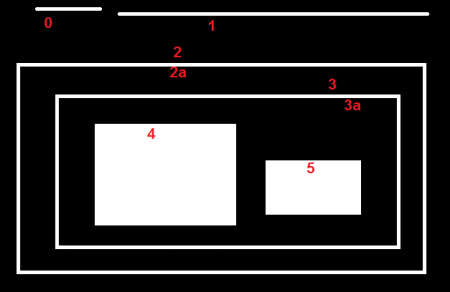
\includegraphics{cont1.png}
\caption{Hierarchy}
\end{figure}

In this image, there are a few shapes which we have numbered from 0 to
5. 2 and 2a denote the external and internal contours of the outermost
box.\\
Here, contours 0,1,2 are external or outermost. We can say, they are in
hierarchy-0 or simply they are in same hierarchy level.\\
Next comes contour-2a. It can be considered as a child of contour-2 (or
in opposite way, contour-2 is parent of contour-2a). So let it be in
hierarchy-1. Similarly contour-3 is child of contour-2 and it comes in
next hierarchy. Finally contours 4,5 are the children of contour-3a, and
they come in the last hierarchy level. From the way I numbered the
boxes, I would say contour-4 is the first child of contour-3a (It can be
contour-5 also).

\section{Hierarchy representation}\label{hierarchy-representation}

Each hierarchy of a contour can be represented by:\\
\texttt{{[}Next,\ Previous,\ First\ Child,\ Parent{]}}\\
\textbf{Next} denotes next contour at the same hierarchical level.\\
\textbf{Previous} denotes previous contour at the same hierarchical
level\\
\textbf{First\_Child} denotes its first child contour.\\
\textbf{Parent} denotes index of its parent contour.\\
For eg, take \textbf{contour-0} in the above picture. Who is next
contour in its same level ? It is contour-1. So simply put Next = 1.\\
Similarly for \textbf{contour-1}, next is contour-2. So Next = 2.\\
What about \textbf{contour-2}? There is no next contour in the same
level. So simply, put Next = -1.\\
What about \textbf{contour-4}? It is in same level with contour-5.So its
next contour is contour-5, so Next = 5.\\
And so on for the others\ldots{}..

\section{Contour retrieval mode}\label{contour-retrieval-mode}

\begin{enumerate}
\def\labelenumi{\arabic{enumi}.}
\tightlist
\item
  \textbf{RETR\_LIST} - retrieves all of the contours without
  establishing any hierarchical relationships.\\
\item
  \textbf{RETR\_EXTERNAL} retrieves only the extreme outer contours. It
  sets hierarchy{[}i{]}{[}2{]} = hierarchy{[}i{]}{[}3{]} = -1 for all
  the contours.\\
\item
  \textbf{RETR\_CCOMP} - This flag retrieves all the contours and
  arranges them to a 2-level hierarchy. ie external contours of the
  object (ie its boundary) are placed in hierarchy-1. And the contours
  of holes inside object (if any) is placed in hierarchy-2. If any
  object inside it, its contour is placed again in hierarchy-1 only. And
  its hole in hierarchy-2 and so on.\\
  We can explain it with a simple image. Here we have labelled the order
  of contours in red color and the hierarchy they belongs to, in green
  color (either 1 or 2).
\end{enumerate}

\begin{figure}[htbp]
\centering
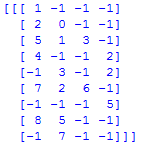
\includegraphics{ccomp.png}
\caption{RETR\_CCOMP}
\end{figure}

\begin{enumerate}
\def\labelenumi{\arabic{enumi}.}
\setcounter{enumi}{3}
\tightlist
\item
  \textbf{RETR\_TREE} - It retrieves all the contours and creates a full
  family hierarchy list.
\end{enumerate}

\begin{figure}[htbp]
\centering
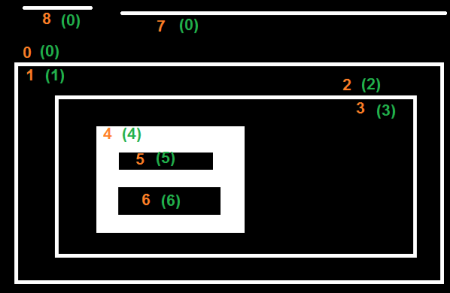
\includegraphics{tree_hierarchy.png}
\caption{RETR\_TREE}
\end{figure}

\section{Code}\label{code}

\begin{verbatim}
  #Importing modules
  import cv2
  import numpy as np
  import matplotlib.pyplot as plt

  #Read the image from the camera
  img1 = cv2.imread('heirarchy.png')
  img2 =  img1.copy()   #Using the same image by copying
  img3 =  img1.copy()
  img4 =  img1.copy()

  #Converting to grayscale
  gray = cv2.cvtColor(img1, cv2.COLOR_BGR2GRAY)

  #Thesholding
  ret,thresh = cv2.threshold(gray,200,255,0)

  #Finding contours for each of them
  contours1,heirarchy1 = cv2.findContours(thresh,cv2.RETR_CCOMP, cv2.CHAIN_APPROX_SIMPLE)
  contours2, heirarchy2 = cv2.findContours(thresh, cv2.RETR_LIST, cv2.CHAIN_APPROX_SIMPLE)
  contours3,heirarchy3 = cv2.findContours(thresh,cv2.RETR_TREE, cv2.CHAIN_APPROX_SIMPLE)
  contours4, heirarchy4 = cv2.findContours(thresh, cv2.RETR_EXTERNAL, cv2.CHAIN_APPROX_SIMPLE)

  #Drawing contours for all of them
  cv2.drawContours(img1, contours1, -1, (0,255,0),1)
  cv2.drawContours(img2, contours2, -1, (0,255,0),1)
  cv2.drawContours(img3, contours3, -1, (0,255,0),1)
  cv2.drawContours(img4, contours4, -1, (0,255,0),1)

  #Printing their hierarchy/ order of relationship
  print heirarchy1
  print heirarchy2
  print heirarchy3
  print heirarchy4

 #Plotting the image 
 plt.subplot(221),plt.imshow(img1),plt.title("RETR_CCOMP")
 plt.xticks([]),plt.yticks([])
 plt.subplot(222),plt.imshow(img2),plt.title("RETR_LIST")
 plt.xticks([]),plt.yticks([])
 plt.subplot(223),plt.imshow(img3),plt.title("RETR_TREE")
 plt.xticks([]),plt.yticks([])
 plt.subplot(224),plt.imshow(img4),plt.title("RETR_EXTERNAL")
 plt.xticks([]),plt.yticks([])
 plt.show()


 #Escape sequence
 cv2.waitKey(0)
 cv2.destroyAllWindows()
\end{verbatim}

The output will be as follows:

\begin{figure}[htbp]
\centering
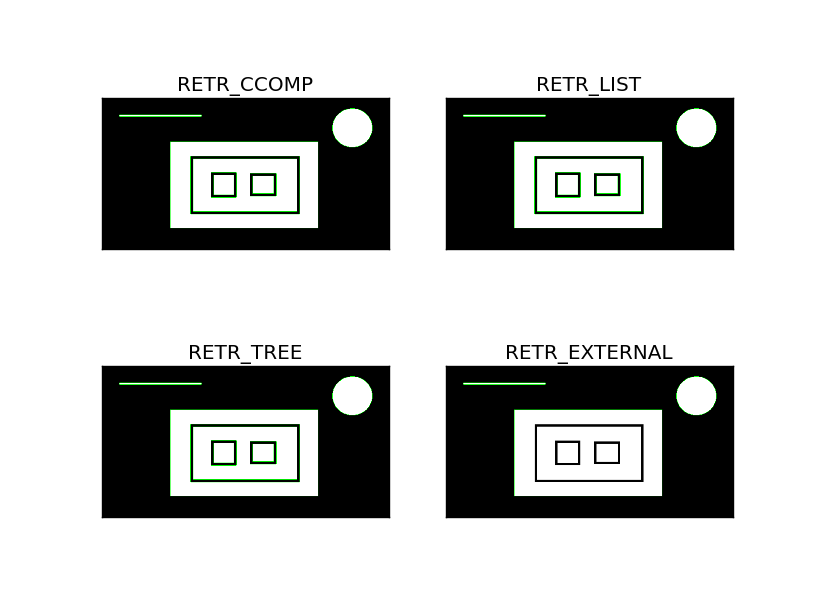
\includegraphics{heir1.png}
\caption{Output}
\end{figure}

We observe that LIST, TREE and CCOMP draw contours the same way. However
the naming of contours differs as you see in the figure below:\\
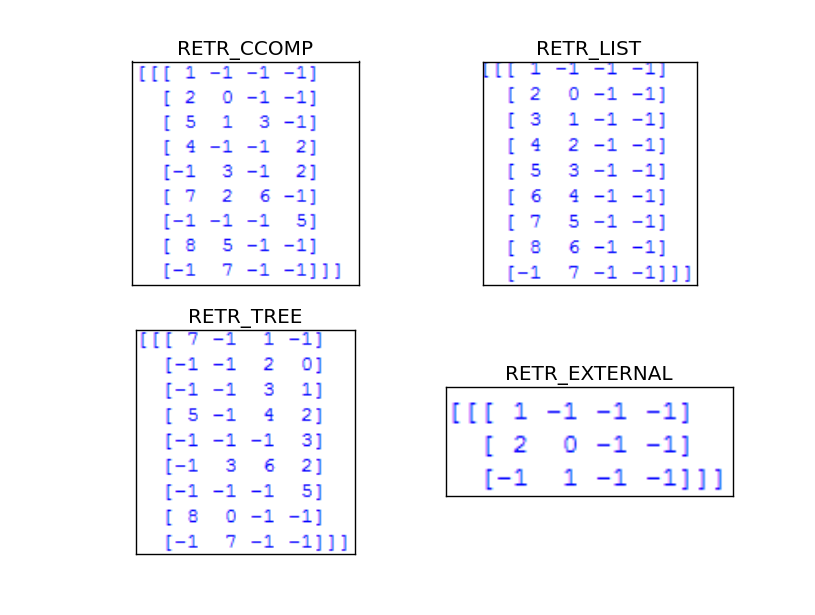
\includegraphics{heir2.png} \\

\LARGE{\textbf{Resources}} \\
\\
1. \href{http://docs.opencv.org/modules/imgproc/doc/structural
\_analysis\_and\_shape\_descriptors.html\#findcontours}{Find contours - opencv docs} \\
2. \href{http://docs.opencv.org/trunk/d9/d8b/tutorial\_py\_contours
\_hierarchy.html}{Contours and hierarchy - opencv docs} \\
3. \href{http://opencv-python-tutroals.readthedocs.org/en/latest/py
\_tutorials/py\_imgproc/py\_contours/py\_contours\_begin/py
\_contours\_begin.html\#contours-getting-started}{Contours - introduction}

\end{document}
